\documentclass{beamer}
\usepackage[utf8]{inputenc}

\usetheme{Madrid}
\usecolortheme{default}

%------------------------------------------------------------
%This block of code defines the information to appear in the
%Title page
\title[Final Presentation] %optional
{Caffeine and Memory}

\subtitle{A brief analysis}

\author[Warren Atkison] % (optional)
{Warren Atkison}



\date[\today] % (optional)
{Stats With Apps, April 2024}


%End of title page configuration block
%------------------------------------------------------------



%------------------------------------------------------------
%The next block of commands puts the table of contents at the 
%beginning of each section and highlights the current section:


%------------------------------------------------------------


\begin{document}

%The next statement creates the title page.
\frame{\titlepage}


%---------------------------------------------------------
%This block of code is for the table of contents after
%the title page
\begin{frame}
\frametitle{Introduction}
\begin{itemize}
	
	\item Does drinking caffeine temporarily improve ones short term memory? This will study the relationship between whether a person has just drank caffeine or not and their ability to improve on a memory test. \pause

	\item I conjecture there is an association between people who drank caffeine before a memory test and people who improved on a memory test.

\end{itemize}
\end{frame}

%---------------------------------------------------------


%---------------------------------------------------------
%Changing visibility of the text
\begin{frame}
\frametitle{Data Collection}
First, 80 people were randomly selected from the Island of Puama between the ages of 20 - 50 and given a DMA test. The next day, participants where split into two groups using random assignment. One group drank 250ml of caffeinated coffee before taking the DMA test again, and the other group drank 250ml of decaf coffee. \pause

\begin{itemize}
    \item Observational units: People from the town of Pauma. \pause
    \item Explanatory variable: Whether a person had caffeine or not for the post treatment test (categorical) \pause
    \item Response variable: Whether or not a person improved from the base-line to post-treatment test (categorical) \pause
    \item It was difficult obtaining consent for 80 Islanders, and getting a wide age range.
\end{itemize}
\end{frame}

%---------------------------------------------------------


%---------------------------------------------------------
%Example of the \pause command
\begin{frame}
\frametitle{Descriptive Statistics}
In the control group (no caffeine), 26/40 people improved their scores and in the treatment group (caffeine) 31/40 people improved their scores. This gives as a sample difference proportion of $0.125$.
\begin{center}
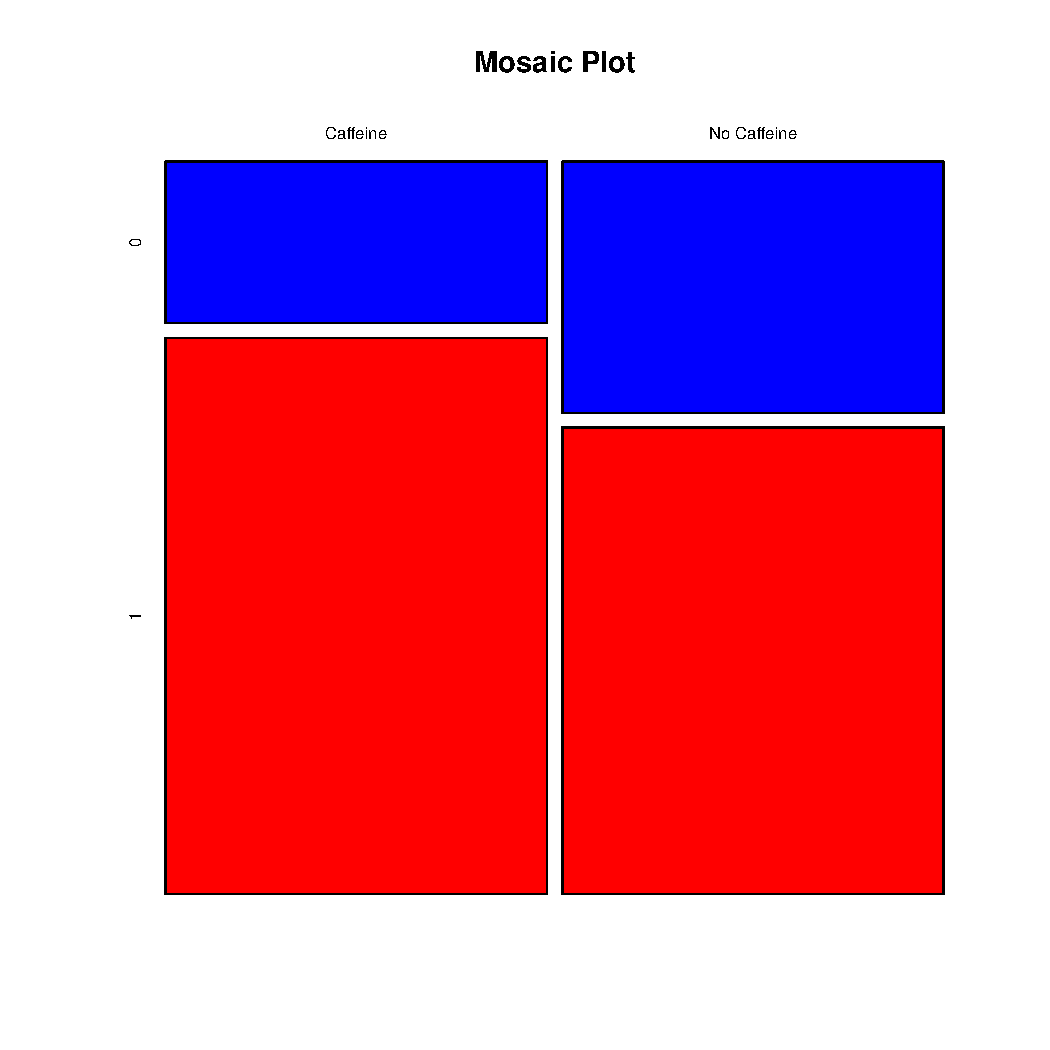
\includegraphics[scale = .3]{Rplots.pdf}
\end{center} \pause
There appears to be a minor or no association.
\end{frame}
%---------------------------------------------------------

\section{Second section}

%---------------------------------------------------------
%Highlighting text
\begin{frame}
\frametitle{Analysis of Results}
Null and alternative hypotheses.
\begin{itemize}
	\item Null hypotheses: The long run difference of proportions of test improvement between the treatment group and control group is zero.
		\[
			H_0: \pi_t - \pi_c = 0.
		\] \pause
	\item Alternative hypotheses: The long run difference of proportions of the treatment group is greater than the long run proportion of the control group.
		\[
			H_a: \pi_t - \pi_c > 0.
		\] \pause
\end{itemize}
Since we used random sampling and random assignment, our measurements are a representative sample of people from the town of Pauma.
\end{frame}
%---------------------------------------------------------


%---------------------------------------------------------
%Two columns
\begin{frame}
\frametitle{Theory Based Approach}
Since we don't have at least 10 samples in each of our categories, namely only 9 people in the treatment group did not improve their test results, a theory based approach is not valid. Regardless, \pause
\begin{itemize}
	\item $z$-score: $z = 1.235$ \pause
	\item One sided p-value: $p = 0.107$ \pause
\end{itemize}
Assuming the null hypotheses, there is a 0.107 probability of achieving this statistic which is greater than 0.05, so we fail to reject the null. We have no evidence that drinking caffeine leads to an improvement in short term memory.
\end{frame}
%---------------------------------------------------------
\begin{frame}
\frametitle{Simulation Based Approach}
Since our validity conditions were not met for the theory based approach, we can do a simulation based approach instead to perform an analysis. \pause
\begin{center}
	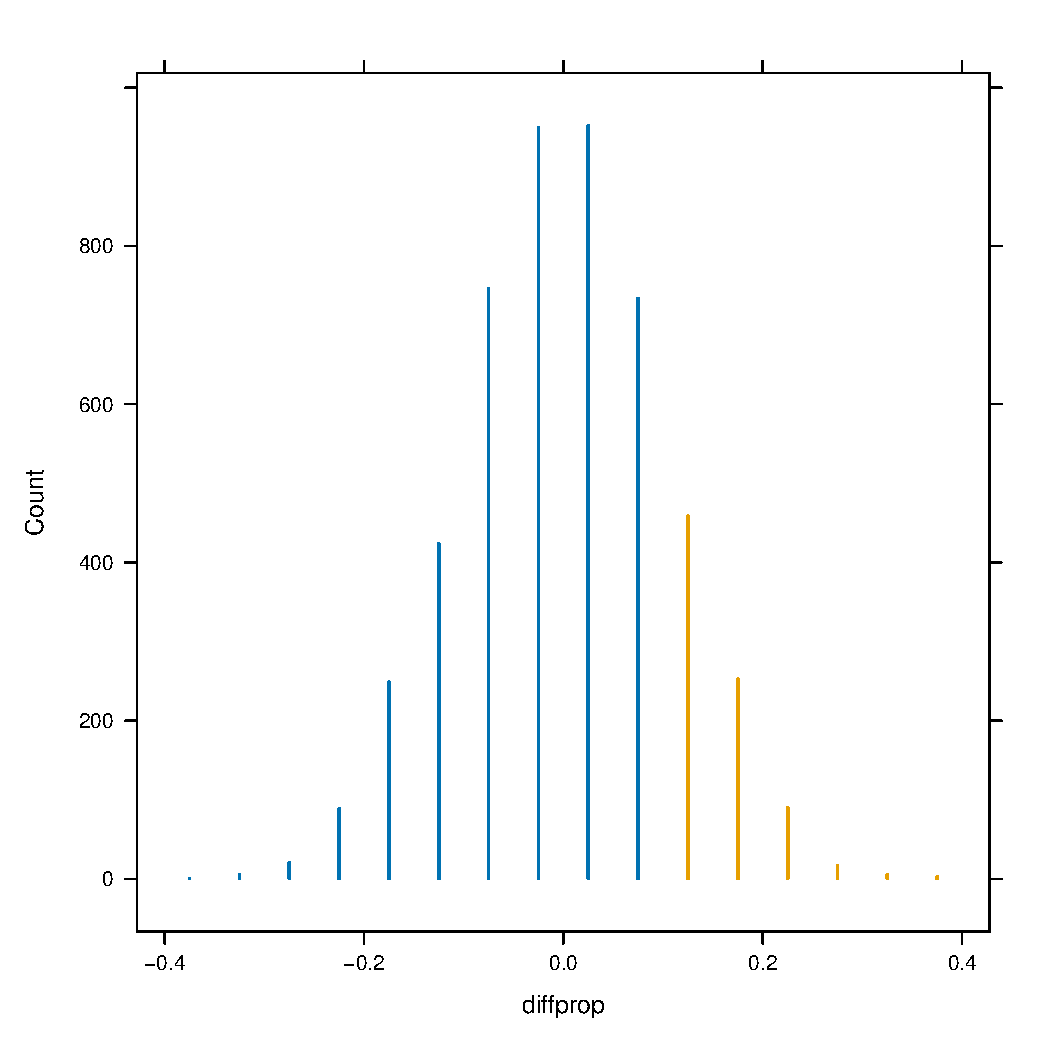
\includegraphics[scale=0.28]{Sim.pdf}
\end{center}
The mean is $0.001$. With our statistic of $31/40 - 26/40 = 0.125$, and a standard deviation $0.102$, we have a $z$-score of $z = 0.125/0.102 = 1.225$
\end{frame}
\begin{frame}
\frametitle{Simulation Based Approach Cont.}
With a $z$-score of $1.225$, we have a $p$-value of $0.110$. This is very similar to our theory based approach despite the validity conditions not being met.
To find a $95\%$ confidence interval, we take 
\[
	(\hat{p}_t - \hat{p}_c) \pm \sigma = 0.125 \pm 0.102
\]
Giving us a confidence interval of $[-0.079,0.329]$. \pause
\begin{itemize}
	\item We are $95\%$ confidant that our parameter for the difference of proportions from the treatment and control is within the interval $[-0.079,0.329]$. Since this interval contains 0, we fail to reject the null.
\end{itemize}
\end{frame}

\begin{frame}
\frametitle{Discussion and Critique}

We have no evidence that taking caffeine before a memory test is associated with improvement in that memory test, since in out simulated analysis we had a 0.110 probability of producing our statistic assuming there is no association which is not statistically significant. \\ \pause
\vspace{10pt}
This did not behave as expected, as I assumed there would be an association. Had there been and association we could have drawn causation as we used random assignment. This data should probably not be generalized to all Islanders, since I only collected data from Pauma. \\ \pause
\vspace{10pt}
Next I would collect a bigger and more representative sample size. A further study could collect a quantitative response variable to measure memory for more in depth analysis.
\end{frame}


\end{document}
